\documentclass{report}

\input{~/latex/template/preamble.tex}
\input{~/latex/template/macros.tex}

\title{\Huge{Chapter  R Notes (Review on Functions)}}
\author{\huge{Matt Warner}}
\date{\huge{}}
\pagestyle{fancy}
\fancyhf{}
\rhead{Math 211 - Calculus and its Applications}
\lhead{\leftmark}
\cfoot{\thepage}
% \usepackage[default]{sourcecodepro}
% \usepackage[T1]{fontenc}
% Tcolorbox setting
\usepackage{tikz}
\usepackage{pgfplots}
\pgfplotsset{compat=1.18}

\pgfpagesdeclarelayout{boxed}
{
  \edef\pgfpageoptionborder{0pt}
}
{
  \pgfpagesphysicalpageoptions
  {%
    logical pages=1,%
  }
  \pgfpageslogicalpageoptions{1}
  {
    border code=\pgfsetlinewidth{1.5pt}\pgfstroke,%
    border shrink=\pgfpageoptionborder,%
    resized width=.95\pgfphysicalwidth,%
    resized height=.95\pgfphysicalheight,%
    center=\pgfpoint{.5\pgfphysicalwidth}{.5\pgfphysicalheight}%
  }%
}
\pgfpagesuselayout{boxed}

\begin{document}
  \maketitle

  \begin{large}
  \textbf{\section{Section R.2}}
  \bigbreak \noindent
  \thmcon{
    \textbf{\underline{Functions and Models}}
    \vspace{3mm}

    A \textbf{\textit{Function} is a correspondence between a first set, called the \textit{domain}, and a second set, called the \textit{range}, such that each member of the domain corresponds to \textit{exactly one} member of the range.}
    \vspace{3mm}

  A function is a special kind of correspondence between two sets that is a fundamental concept in mathematics. Consider the following situations. 
  \vspace{3mm}
  \begin{itemize}
    \item For each weekday, there corresponds the closing value of the Dow Jones Industrial Average.
    \item For each student  at a univeristy, there corresponds the student's identification number.
    \item For each letter on a phone's keypad, there corresponds a number.
    \item For each real number $x$, there corresponds that number's square, $x^{2}$.
  \end{itemize}
\vspace{4mm}

In each of these examaples, the first set is called the \textit{domain} and the second set is called the \textit{range}. For any member of the domain, there is \textit{exactly one} member of the range to which it corresponds (is matched). This type of correspondence is called a \textit{function}.

  }
  \end{large}
\bigbreak \noindent \bigbreak \noindent
\ex{}{
  Determine whether or not each correspondence is a function. (Shown in the figure below.)
  \vspace{3mm}
}
\begin{figure}[ht]
\centering
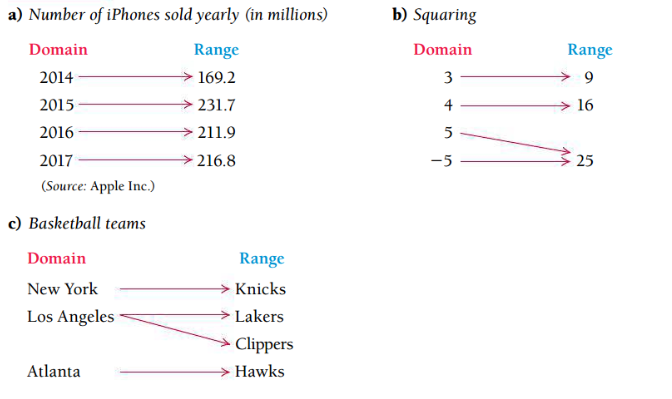
\includegraphics[width=0.7\textwidth]{ ksnip_20230829-130232.png }
\end{figure}
\pagebreak
\pf{Solution to Example 0.1.1}

\vspace{3mm}

\noindent \textbf{a)} The correspondence is a function because each member of the domain corresponds to only one member of the range.
\vspace{3mm}

\noindent \textbf{b)} The correspondece is a function becuase each member of the domain corresponds to only one member of the range, even though two members of the domain correspond to 25.
\vspace{3mm}

\noindent \textbf{c)} The correspondence is \textit{not} a function becuase one member of the domain, Los Angeles, corresponds to two members of the range, Lakers and Clippers.
\bigbreak \noindent \bigbreak \noindent
\ex{} {
  \vspace{3mm}

  Determine whether or not each correspondence is a function.
}
\vspace{2mm}

\begin{figure}[ht]
\centering
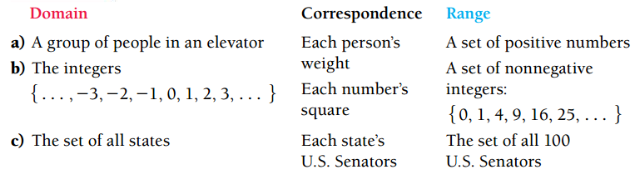
\includegraphics[width=0.75\textwidth]{ example2.png }
\end{figure}
\bigbreak \noindent
\pf{Solution to Example 0.1.2}

\noindent \textbf{a)} The correspondece is a function becuase each person has \textit{only one} weight.
\vspace{3mm}

\noindent \textbf{b)} The correspondence is a function becuase each integer has \textit{only one} sqaure.
\vspace{3mm}

\noindent \textbf{c)} The correspondence is \textit{not} a function because each state has \textit{two} U.S Senators.

\bigbreak \noindent \bigbreak \noindent
Consistent with the definition on p.13, we can regard a function as a set of ordered pairs, such that no two pairs have the same first coordinate paired with different second coordinates. When a function is written as a set of ordered pairs, the domain is the set of all first coordinates, and the range is the set of all second coordinates. Function names are usually represented by lowercase letters. Thus, if $f$ represents the function in Example 2(b), we have.
\vspace{3mm}

$$ f = {\ \ldots, (-3,9), (-2,4), (-1,1),(0,0),(1,1),(2,4),(3,9),\ldots}\}$$
and,
\vspace{2mm}

domain of $f$ = \{\ \ldots, $-3,-2,-1,0,1,2,3,\ldots\}$; range of $f = {\ 0,1,4,9,\ldots}\} $
\pagebreak
\thmcon{
  \textbf{\underline{Finding Function Values}}
  \vspace{3mm}

  \noindent Functions can be described by equations such as $y=2x+3$ and $y=4-x^2$. To graph the function given by $y=2x+3$, we find ordered pairs by performing calculations for selected x values:
  \vspace{3mm}

  \begin{center}
    for $x = 4, y = 2 \cdot 4 + 3 = 11$; \hspace{5mm} The graph includes $(4,11)$
    \vspace{2mm}

    for $x = -5, y \cdot (-5) + 3 = -7$; \hspace{5mm} The graph includes $(-5,-7)$
    \vspace{2mm}

    for $x=0,y=2 \cdot 0 + 3 = 3$; and so on. \hspace{5mm} The graph includes $(0,3)$.

    
  \end{center}
  \bigbreak \noindent
  The inputs (members of the domain) are the values of $x$ substitued into the equation. The outputs (memebers of the range) are the resulting values of y. If we call the function $f$, we can use $x$ to represent an arbitrary input and $f(x)$, read ``$f$ of $x$'' or ``$f$ at $x$''or ``the value of $f$ at $x$,'' to represent the corresponding output. In this notation, the function given by $ y=2x+3$ is written as $f(x) = 2x+3$, and the calculations above can be written more concisely as
  $$f(4) = 2 \cdot 4 + 3 = 11;$$ 
  $$ f(-5) = 2 \cdot (-5) + 3 = -7;$$
  $$ f(0) = 2 \cdot 0 + 3 = 3;$$
}
\bigbreak \noindent \bigbreak \noindent
\ex{}{

  The squaring function $f$ is given by $f(x) = x^2$. Find $f(-3), f(1), f(k), f(\sqrt{k})$, and $f(x+h)$.
}
\bigbreak \noindent
\pf{Solution to above problem}

We have,
$$ f(-3) = (-3)^2 = 9;$$ 
$$f(1) = 1^2 = 1;$$
$$f(k) = k^2;$$
$$f(\sqrt{k}) = (\sqrt{k})^2 = k;$$
$$ f(x+h) = (x+h)^2 = x^2 = 2xh + h^2$$.
\bigbreak \noindent \bigbreak \noindent
\ex{}{
  
  A function $g$ is given by $g(x) = 3x^2 - 2x+8.$ Find $g(0), g(-5),$ and $g(7a)$.
}
\bigbreak \noindent
\pf{Solution to above problem:}

We Have,
$$ g(0) = 3 \cdot 0^2 - 2 \cdot 0 + 8 = 8 $$
$$ g(-5) = 3(-5)^2 -2 \cdot (-5)+ 8 = 3 \cdot 25 + 10 + 8 = 75 + 10 + 8 = 93.$$
$$g(7a) = 3(7a)^2 - 2(7a) + 8 = 3 \cdot 49a^2 - 14a + 8 = 147a^2 - 14a +8$$
\pagebreak
\ex{}{

  A function $f$ subtracts the square of an input from the input:
  $$ f(x) = x-x^2$$
  Find $f(4), f(x+h)$, and $\frac{f(x+h) -f(x)}{h}$
}
\pf{Solution to above problem}

We have,
$$f(4) = 4 - (4)^2 = 4 -16 = -12$$

$$f(x+h) = (x+h) - (x+h)^2 =  x+h - (x^2 + 2xh + h^2) = x+h - x^2 - 2xh - h^2$$

$$\frac{f(x+h)-f(x)}{h}  =\frac{x_{x+h-x^2-2 x h-h^2}-{\left(x-x^2\right)}}{h}$$
$$ =\frac{h-2 x h-h^2}{h} \quad \text { Simplifying }$$
$$ =\frac{h(1-2 x-h)}{h} \quad \text { Factoring } $$
$$ =1-2 x-h, \quad \text { for } h \neq 0$$

\bigbreak \noindent \bigbreak \noindent
\thmcon{
  \textbf{\underline{Graphs of Functions}}
  \vspace{3mm}

  The \textbf{graph} of a function $f$ is a drawing that represents all the input-output pairs, $(x,f(x))$. When the function is given by an equation, the graph of the function is the graph of the equation, $y=f(x)$.
  \vspace{3mm}
  
  It is customary to locate input values (the domain) on the horizontal axis and output values (the range) on the vertical axis.

}
\bigbreak \noindent
\ex{}{
  
  \centering{Graph $f(x) = x^2 + 1$}

}
\pf{Solution for Example 0.1.6}

\noindent % This prevents indentation of the first line
\begin{minipage}{0.5\textwidth}
  \centering % Centers the content
  \[
  \begin{array}{|r|r|r|}
    \hline
    \multicolumn{1}{|c|}{x} & \multicolumn{1}{c|}{f(x)} & \multicolumn{1}{c|}{(x, f(x))} \\
    \hline
    -2 & 5 & (-2,5) \\
    -1 & 2 & (-1,2) \\
    0 & 1 & (0,1) \\
    1 & 2 & (1,2) \\
    2 & 5 & (2,5) \\
    \hline
  \end{array}
  \]
\end{minipage}%
\hspace{-0.1\textwidth}% Space between minipages
\begin{minipage}{0.45\textwidth}
  \centering % Centers the content
  \begin{tikzpicture}
    \begin{axis}[
      restrict y to domain=-6:6,
      restrict x to domain=-6:6,
      samples=200,
      xmin=-6,
      xmax=6,
      ymin=-6,
      ymax=6,
      axis lines=middle,
      xlabel={\(x\)},
      ylabel={\(y\)},
    ]
      \addplot[color=red]{x^2+1};
    \end{axis}
  \end{tikzpicture}
\end{minipage}
\pagebreak
\begin{large}
  \textbf{\section{Functions Defined Piecewise}} 
\end{large}
\bigbreak \noindent
\thmcon{
  \textbf{\underline{Defintion}}
  \vspace{3mm}

  Some functions are defined \textit{piecewise}, using different output formulas for different parts of the domain. To graph a piecewise-defined function, we use the correspondence specified for each part of the domain.
  
}
\bigbreak \noindent
\begin{large}
\noindent \textbf{Example:} 
\end{large}
\begin{center}
\[
f(x) = 
\begin{cases} 
  4 & \text{for} x \le 0, \\
  3-x^2 & \text{for } 0 < x \ge 2, \\
  2x-6 & \text{for} x > 2
\end{cases}
\] 
\end{center}
\vspace{5mm}

\noindent Working from left to right, note that for all x-values less than or equal to 0, the graph is the horizontal line y = 4. 
\vspace{2mm}

\noindent For example,

$$ f(-2) = 4;$$
$$ f(-1) =4;$$
$$ f(0) = 4;$$
\bigbreak \noindent \bigbreak \noindent
\ex{}{

  Graph the function defined as follows:
  \vspace{3mm}
  \[
  g(x) = 
  \begin{cases}
    3, & \text{for } x = 1 \\
    -x + 2, & \text{for } x \neq 1 
  \end{cases}
  \]
}
\bigbreak \noindent
\pf{Solution: }

The function is defined such that $g(1) = 3$ and for all other x-values (that is, for $x \neq 1$), we have $g(x) = -x + 2$. Thus, to graph this function, we have the line given by $y = -x + 2$, but with an open dot at the point corresponding to $x = 1$ To complete the graph, we plot the point $(1,3)$ since $g(1) = 3$.
\bigbreak \noindent
\begin{minipage}{0.5\textwidth}
  \centering % Centers the content
  \[
  \begin{array}{|r|r|r|}
    \hline
    \multicolumn{1}{|c|}{x} & \multicolumn{1}{c|}{f(x)} & \multicolumn{1}{c|}{(x, f(x))} \\
    \hline
    -3 & -(-3) + 2 & (-3,5) \\
    0 & -0 + 2 & (0,2) \\
    1 & 3 & (1,3) \\
    2 & -2 + 2 & (2,0) \\
    3 & -3 + 2 & (3,-1) \\
    \hline
  \end{array}
  \]
\end{minipage}%
\hspace{-0.1\textwidth}% Space between minipages
\begin{minipage}{0.45\textwidth}
  \centering % Centers the content
\begin{tikzpicture}
\begin{axis}[
    axis lines = middle,
    xlabel = \(x\),
    ylabel = \(y\),
    xmin = -1, xmax = 3,
    ymin = -1, ymax = 4,
    samples = 200
]
% Plot the function for x not equal to 1
\addplot[domain=-1:0.99, blue] {-x + 2};
\addplot[domain=1.01:3, blue] {-x + 2};

% Plot the point for x = 1
\addplot[only marks, mark = *, red] coordinates {(1, 3)};

% Label the point (1, 3)
\node[red, right] at (axis cs: 1, 3) {(1, 3)};

\end{axis}
\end{tikzpicture}
\end{minipage}
\pagebreak
\begin{large}
  \textbf{\section{\LARGE{Finding Domain and range}}}
  \bigbreak \noindent
  \textbf{Set Notation}
\end{large}
\bigbreak \noindent
\thmcon{
  \textbf{\underline{Defintion}}
  \vspace{3mm}

  A set is any collection of objects, such as numbers. The set of numbers we consider most often in calculus is the set of real numbers, denoted $\mathbb{R}$. The real numbers can be represented by a line, called the \textbf{real number line}. Every point on the line represents a real number. 
  \bigbreak \noindent
For example, the set consisting of \{$2, -\frac{1}{2}, \pi$\}. On the real number line, a dot is placed at each number's location:
\bigbreak \noindent
\begin{center}
  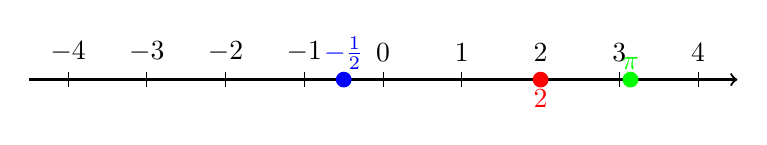
\begin{tikzpicture}
    % Draw the main number line
    \draw[thick, ->] (-4.5,0) -- (4.5,0);
    % Draw the tick marks and labels
    \foreach \x in {-4,-3,-2,-1,0,1,2,3,4} {
        \draw (\x,-0.1) -- (\x,0.1) node[above] {\(\x\)};
    }
    % Add custom points
    \fill[red] (2,0) circle (0.1);
    \node[below, red] at (2,0) {\(2\)};
    
    \fill[blue] (-0.5,0) circle (0.1);
    \node[above, blue] at (-0.5,0) {\(-\frac{1}{2}\)};
    
    \fill[green] ({pi},0) circle (0.1);
    \node[above, green] at ({pi},0) {\(\pi\)};
\end{tikzpicture}
\end{center}
\bigbreak \noindent
This method of describing a set by listing its members within braces \{ \} is known as the \textbf{roster method} Larger sets can be described using \textbf{set-builder notation}, which specifies conditions for which an object is a member of the set. For example, the set of all real numbers less than 4 can be described in set-builder notation as follows:

}
\bigbreak \noindent \bigbreak \noindent
\begin{large}
 \textbf{Interval Notation}
\end{large}
\thmcon{
  \textbf{\underline{Defintion}}
  \vspace{3mm}

  We can also describe certain sets using \textbf{interval notation}. If $a$ and $b$ are \textit{real numbers}, with $a<b$, we define the interval \textit{a,b} as the set of all numbers between but not including $a$ and $b$, that is, the set of all $x$ for which $a<x<b$.
  \vspace{2mm}

  Thus,
  \begin{center}
    the set $(a,b)$ = $\{x|a < x < b\}$ is displayed on the number line as:
    \vspace{2mm}

    \begin{tikzpicture}
  % Draw the number line
  \draw[->, thick] (0,0) -- (10,0);
  
  % Draw labels and ticks for 'a' and 'b'
  \draw (2,0.2) -- (2,-0.2);
  \node[below] at (2,-0.2) {\(a\)};
  \draw (8,0.2) -- (8,-0.2);
  \node[below] at (8,-0.2) {\(b\)};
  
  % Draw opening parenthesis facing right for 'a'
  \node at (2,0) {\textbf{(}};
  
  % Draw closing bracket facing left for 'b'
  \node at (8,0) {\textbf{]}};
  
  % Draw red line from 'a' to 'b'
  \draw[red, thick] (2,0) -- (8,0);
  
\end{tikzpicture}

  \end{center}

}
\nt{

  The points \textit{a} and \textit{b} are the \textbf{endpoints} of the interval. The parentheses indicate that the endpoints are not included in the interval.
  \vspace{2mm}

  the set [a, b] = $\{x|a < x \ge b\}$
  \begin{center}
    \begin{tikzpicture}
  % Draw the number line
  \draw[->, thick] (0,0) -- (10,0);
  
  % Draw labels and ticks for 'a' and 'b'
  \draw (2,0.2) -- (2,-0.2);
  \node[below] at (2,-0.2) {\(a\)};
  \draw (8,0.2) -- (8,-0.2);
  \node[below] at (8,-0.2) {\(b\)};
  
  % Draw opening parenthesis facing right for 'a'
  \node at (2,0) {(};

  % Draw closing bracket facing left for 'b'
  \node at (8,0) {]};
  
  % Draw red line from 'a' to 'b'
  \draw[red, thick] (2,0) -- (8,0);
\end{tikzpicture}
  \end{center}
}
\bigbreak \noindent \bigbreak \noindent
\begin{large}
  \textbf{Union and Intersection of Intervals} 
\end{large}
\thmcon{
  \textbf{\underline{Defintion (Union)}}
  \vspace{3mm}
  
  The \textit{union} of two (or more) intervals consists of all real numbers $x$ that are contained in one interval \textit{or} the other \textit{or} both. We use the symbol $\cup$ to represent the union of intervals. For example, $[2,1) \cup [4,7]$ represents all real numbers x such that $-2 \ge x < 1$ \textit{or} $ 4\ge x\ge 7 $.
  \vspace{2mm}
}
\pagebreak

 \begin{figure}[ht]
   \hspace{27mm}
 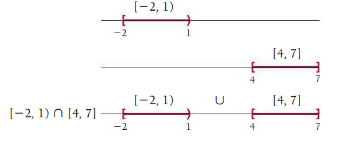
\includegraphics[width=0.6\textwidth]{ cup.png }
 \caption{Example of Union}
 \end{figure} 
\bigbreak \noindent
\thmcon{
  \textbf{\underline{Defintion}}
  \vspace{3mm}

  The \textit{intersection} of two (or more) intervals consists of all real numbers $x$ that are contained in both (or all) intervals simultaneously. We use the symbol $\cap$ to represent the intersection of intervals. For example, $(0,5) \cap [2,7)$ represents all real numbers $x$ such that $0<x<5$ \textit{and} $2 \ge x 7$, and simplifies as the interval $[2,5]$.

}
  \begin{figure}[ht]
    \hspace{32mm}
  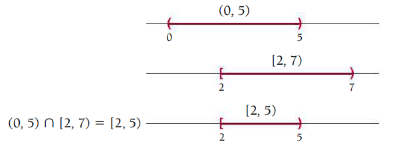
\includegraphics[width=0.5\textwidth]{ cap.png }
  \caption{Example of Intersection} 
  \end{figure}
\bigbreak \noindent
\nt{
  When two intervals do not contain any common elements, then their intersection is empty, denoted by $\emptyset$  
  \vspace{2mm}

  For example, the interval $[-2,1) \text{and} [4,7]$ shown above do not have any real numbers in coomon (numbers that are in both intervals simultaneously), so $[-2,1] \cap [4,7] = \emptyset$. Such intervals are called \textit{disjoint}
}
\bigbreak \noindent


\ex{}{
Write interval notation for each set or graph:
}  
\bigbreak \noindent\bigbreak \noindent
  \begin{figure}[ht]
  \centering
  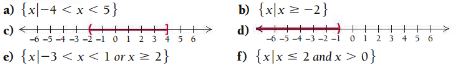
\includegraphics[width=0.8\textwidth]{ example3.png }
  \end{figure}
\pagebreak

\begin{problemset}{Example 0.3.1 solutions}
\begin{align*}
\prob{a} & \sol{(-4,5)}      & \prob{b} & \sol{[-2,\infty]}       & \prob{c} & \sol{(-2,4]}         \\
\prob{d} & \sol{(-\infty, -1)}  & \prob{e} & \sol{(-3,1) \cup [2,\infty]}  & \prob{f} & \sol{(0,\infty)}  
\end{align*}
\end{problemset}
\hrule
\begin{large}
  \textbf{\subsection{Finding Domain and Range}} 
\end{large}
\bigbreak \noindent
Recall that a set of ordered pairs in which no two different pairs share a common first coordinate is a function
\vspace{3mm}

\noindent The \textbf{Domain} is the set of all first coordinates, and the \textbf{range} is the set of all second coordinates
\bigbreak \noindent
\ex{}{

\noindent % to prevent indentation of the minipage
\begin{minipage}{0.5\textwidth}
  For the function $f$ shown in the graph \\
  to the right, determine the domain and range.
\end{minipage}%
\begin{minipage}{0.5\textwidth}
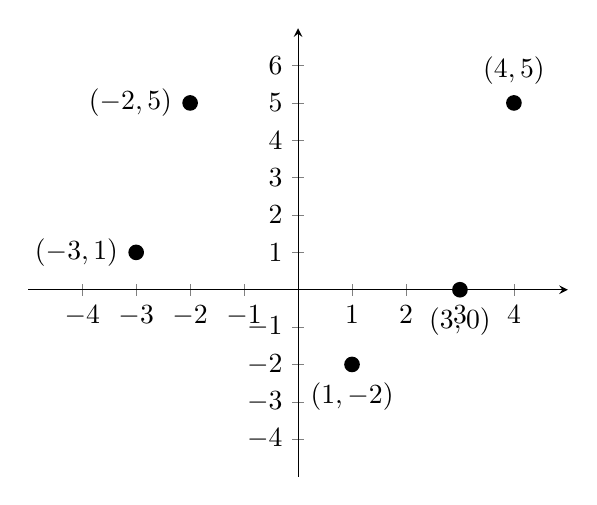
\begin{tikzpicture}
    \begin{axis}[
        axis lines=middle,
        xmin=-5, xmax=5,
        ymin=-5, ymax=7,
        xtick={-4,-3,...,4}, % x ticks
        ytick={-4,-3,...,6}, % y ticks
        ]
        \addplot[only marks] coordinates {(-3,1) (-2,5) (1,-2) (3,0) (4,5)};
        
        % Labels
        \node[label={180:$(-3,1)$},circle,fill,inner sep=2pt] at (axis cs:-3,1) {};
        \node[label={180:$(-2,5)$},circle,fill,inner sep=2pt] at (axis cs:-2,5) {};
        \node[label={270:$(1,-2)$},circle,fill,inner sep=2pt] at (axis cs:1,-2) {};
        \node[label={270:$(3,0)$},circle,fill,inner sep=2pt] at (axis cs:3,0) {};
        \node[label={90:$(4,5)$},circle,fill,inner sep=2pt] at (axis cs:4,5) {};
    \end{axis}
\end{tikzpicture}
\end{minipage}
}
\bigbreak \noindent
\begin{problemset}{Example 3.2 Solution}
\begin{align*}
  \text{ Domain: }\{-3,-2,1,3,4\} \hspace{5mm} \text{Range: }\{-2,0,1,5\}
\end{align*}
\end{problemset}
\bigbreak \noindent
\nt{
  Recall that a denominator cannot equal zero. So when finding the domain of a rational function, setting the denomiator equal to 0 will give you want is not to be included in the domain.
  \vspace{3mm}

  For instance,
  $$ \frac{3}{2x-5}$$

  Set the denomiator equal to 0 and solve.
  $$ 2x - 5 = 0 \rightarrow x = \frac{5}{2}$$
  
  In this example, $\frac{5}{2}$ cannot be in the domain, so the domain is $(-\infty, \frac{5}{2}) \cup (\frac{5}{2}, \infty)$
  \vspace{3mm}

  The domain can also be written as: $\{x | x \neq \frac{5}{2}\}$

}
\pagebreak
\nt{
  Recall that radicands in even roots cannot be negative, $\sqrt{4+3x}$ is not a real number when $4+3x$ is negative.
  \vspace{2mm}

  The domain is all real numbers for which $4+3x \ge 0$
\bigbreak \noindent
  We find the Domain by solving the inequality.
  
  $$4+3x \ge 0$$
  $$3x \ge -4$$
  $$x \ge -\frac{4}{3}$$
\bigbreak \noindent
The domain is $\{x | x -\frac{4}{3} \le x < \infty \}$
}
\bigbreak \noindent \bigbreak \noindent
\ex{}{
  \vspace{3mm}

  Find and graph the domain: $h(x) = \sqrt{x} + \sqrt{3-x}$
}
\vspace{4mm}

\sol{}
\vspace{2mm}

The radicands of both square root terms must be nonnegative.
\vspace{3mm}

So,

$$ \text{\prob{1} }\sqrt{x} \ge 0 = x \ge 0$$
$$\text{\prob{2} } 3-x \ge 0 = x \le 3$$

Therefore, 

$$ \{x | x \ge 0\} \cap \{x|x \le 3\} = [0,3]$$
\vspace{3mm}

\hrule
\bigbreak \noindent
\begin{large}
  \textbf{\subsection{Domains and Ranges in Applications}} 
\end{large}
\bigbreak \noindent
The domain and the range of a function given by a formula are sometimes affected by the contex of an application. In such cases, we consider the function's practical domain and the range.
\vspace{5mm}

For example, for the function $y = 15x$, 
\vspace{2mm}

the domain is $\{x|x \text{ is any real number}\}$ 
\vspace{2mm}

and the range is $\{y|y \text{ is any real number}\}$
\vspace{5mm}

\noindent However, if the function represents the pay, $y$, for someone who works $x$ hours at $\$15$ per hour, then negative values of $x$ and $y$ do not make sense.
\vspace{4mm}

\noindent In this case, the functions practical domain is $\{x|x \ge 0\}$ and its practical range is $\{y|y \ge 0\}$.
\pagebreak

\ex{}{
  \textcolor{blue}{\underline{Rental Car Rates}.} 
  \vspace{2mm}

  The hourly rate to rent a minivan in Florida is $\$12.30$ per hour or any part of an hour.
  \vspace{2mm}

  For any rental period of more than 2 hr, the daily rate of $\$36.90$ applies, up to and including a maximum of 24 hr. This pricing also applies to subsequent 24-hr periods.
  \vspace{5mm}

  Let $C(t)$ be the cost to rent a minivan for $t$ hours. Disregard any extra taxes or surcharges.
  \bigbreak \noindent
  \prob{a} Find $C(18)$, and explain what this number represents.
  \vspace{2mm}

  \prob{b} Find $C(22.5)$, and explain what this number represents.
  \vspace{2mm}

  \prob{c} Find $C(30)$, and explain what this number represents.
  \vspace{2mm}

  \prob{d} Sketch the graph of $C$ for $ 0 < t \le 48$, and state the practical range $C$.
}
\bigbreak \noindent
\sol{}

\bigbreak \noindent
\prob{a} Since 18 hr exceeds 2 hr and is less than 24 hr, we have $C(18) = 36.90$, meaning that the charge to rent a minivan for 18 hr is the daily rate of $36.90$.
\vspace{3mm}

\noindent\prob{b} A rental period of 25.5 hr consists of a 24-hr period for which the daily rate is charged plus two 1-hr periods, since the extra $0.5$ hr is considered part of the full second hr. Thus,
$$C(25.5) = \$36.90 + \$12.30 + \$12.30 = \$61.50$$
\bigbreak \noindent
\prob{c} A rental period of 30 hr consists of a 24-hr period for which the daily rate is charged plus an extra 6 hr for which the daily rate is charged again. Thus,
$$ C(30) = 36.90 + 36.90 = 73.80$$
\bigbreak \noindent
\prob{d} The graph of $C$, for $0 < t \le 48$, is shown below.
\vspace{3mm}
\bigbreak \noindent
\begin{figure}[ht]
\centering
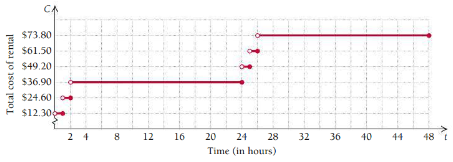
\includegraphics[width=0.74\textwidth]{ dgraph.png }
\end{figure}
\bigbreak \noindent
\pagebreak
\section{R.4 - Slope and Linear Functions}
\bigbreak \noindent
Given any two points $P_1 = (x_2, y_2)$, we can draw a line containing these points. A measure of the line's steepness is called the \textbf{slope}, denoted by the letter $m$.
\bigbreak \noindent \bigbreak \noindent
\thmcon{
  \textbf{\underline{Defintion}}
  \vspace{3mm}

  The \textbf{Slope} of a line containing points $P_1 = (x_1, y_1)$ and $P_2 = (x_2,y_2)$ is

  $$ m = \frac{y_2-y_1}{x_2-x_1} = \frac{\text{change in }y}{\text{change in }x}$$
}
\bigbreak \noindent \bigbreak \noindent
\ex{
\textbf{Find the slope of a line containing the points ($-2,6$) and ($-4,9$)}.
}
\bigbreak \noindent
\sol{We have,}
\bigbreak \noindent
$$ m = \frac{y_2 - y_1}{x_2 - x_1} = \frac{9-6}{-4+2}$$

$$ m = -\frac{3}{2}$$
\bigbreak \noindent
\nt{
  It does not matter which point is regarded as $p_1$ or $p_2$, as long as we subtract the coordinates in the same order. Thus we can also find $m$ as follows:
  $$m = \frac{6-9}{-2+4} = -\frac{3}{2}$$
}
\bigbreak \noindent \bigbreak \noindent
\underline{\textbf{Horizontal and Vertical lines}}
\vspace{1em}

\noindent If a line is horizontal, the vertical change between any two points is 0. Thus, a horizontal line has slope 0. If a line is vertical, the horizontal change between any two points is 0. In this case, the slope is \textit{not defined} because we cannot divde by 0. A vertical line has undefined slope. Thus \textbf{0 slope} and \textbf{undefined slope} are two very different concepts.
\bigbreak \noindent \bigbreak \noindent
\underline{\textbf{Applications of slope}}
\vspace{1em}

\noindent Slope has many real-world applications. For example, numbers like 2\%, 3\%, and 6\% are often used to represent the \textit{grade}, or steepness, of a road. A 3\% grade $\left(3\% = \frac{3}{100}\right)$ means that for every horizontal distance of 100ft, the road rises 3 ft.
\vspace{1em}

\noindent In solar arrays, photovoltaic panels are tilted to optimize solar gain, based on geography and weather patterns. Wheelchair-ramp design also involves slope: Building codes rarely allow the steepness of a wheelchair to exceed $\frac{1}{12}$.
\pagebreak
\ex{}{
  The amount spent on cancer research has increased steadily over the years and is approximated in the graph below. Find the average rate of change of the amount spent on the research.
}
\begin{figure}[ht]
\centering
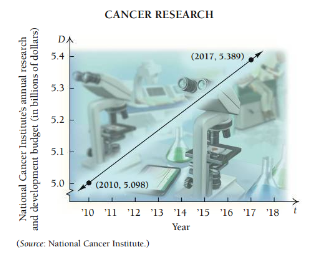
\includegraphics[width=0.5\textwidth]{ slope.png }
\end{figure}
\bigbreak \noindent
\sol{Given the two points shown on the graph, we can use the slope formula}

$$ P_1 = (2010, 5.098) \hspace{1em} P_2 = (2017, 5.389)$$

$$\hspace{-1.5em} M = \left(\frac{5.389 - 5.098}{2017 - 2010}\right)$$

$$ M = \frac{.291}{7} \approx \$0.0416 \text{ billion}$$
\bigbreak \noindent
\hrule
\bigbreak \noindent
\thmcon{
  \textbf{\underline{Defintion}}
  \vspace{3mm}

  In general we have the following,
  \vspace{1em}

  The graph of $y = c $, a horizontal line, is the graph of a function. Such a function is referred to as a \textbf{constant function}
  \vspace{1em}

  The graph of $x = a$ is a vertical line and does not represent a function.
}
\bigbreak \noindent \bigbreak \noindent
  \subsection{Equations of the Form y= mx or y = mx + b}
  \bigbreak \noindent
Consider the following table of numbers and look for a pattern
\bigbreak \bigbreak
\begin{large}
\hspace{9em}\begin{tabular}{|l|l|l|l|l|l|l|l|l|c|}
\hline$x$ & 0 & 1 & -1 & $-\frac{1}{2}$ & 2 & -2 & 3 & -7 & 5 \\
\hline$y$ & 0 & 3 & -3 & $-\frac{3}{2}$ & 6 & -6 & 9 & -21 & 15 \\
\hline
\end{tabular}
\end{large}

\pagebreak
\begin{mdframed}
Note that the ratio of the y-values to x-values is 3 to 1. 
\vspace{1em}

\noindent Thus,

$$ y = 3x$$
\vspace{1em}

\noindent Ordered pairs from the table can be used to graph y = 3x. Note that this is a function and that 3 is the slope between any two pairs of points in the table.
\end{mdframed}
\bigbreak \noindent \bigbreak \noindent
\thmcon{
  \textbf{\underline{Defintion}}
  \vspace{3mm}

  A \textbf{linear function} is any function that can be written in the form

  $$y = mx + b \hspace{5mm} or \hspace{5mm} f(x) = mx+b$$
  \vspace{1em}

  Its graph has the same slope, $m$, as the graph of $y=mx$ and crosses the y-axis at (0,b). This point (0,b) is called the y-intercept.
  \vspace{1em}

  Two lines that have the same slope but different y-intercepts are \textbf{parallel}. The graphs of $y= mx$ and $y=mx+b$ (for b $\neq$ 0) are parallel lines for any value of $m$.

}
\bigbreak \noindent
\hrule
\subsection{The Slope-Intercept Equation}
\bigbreak \noindent
Every nonvertical line is uniquely determined by its slope $m$ and its y-intercept (0,b). In other words, the slope describes the "slant" of the line, and the y-intercept locates the point at which the line crosses the y-axis.
\vspace{3mm}

\noindent Thus, we have the following.
\vspace{2mm}

$$ y = mx+ b \text{ \textbf{slope-intercept equation} of a line.}$$
\bigbreak \noindent \bigbreak \noindent
\ex{}{
  Find the slope and the y-intercept of the graph of: $$2x - 4y - 7 = 0$$
}
\bigbreak \noindent 
\sol{}

$$ 2x-4y-7=0$$

$$2x-7=4y$$

$$\frac{2x}{4} - \frac{7}{4} = y$$

$$y = \frac{1}{2}x - \frac{7}{4}$$

\pagebreak
\subsection{The point-Slope Equation}
\bigbreak \noindent
Suppose we know the slope of a line and any point on the line. We can use these to find an equation of the line.
\bigbreak \noindent \bigbreak \noindent
\ex{}{
  Find an equation of the line with slope 3 containing the point (-1,-5).
}
\bigbreak \noindent
\sol{}
\bigbreak 
\begin{mdframed}
We can use the equation:

$$ y-y_1 = m(x-x_1)$$
\vspace{2mm}

So,

$$ y + 5 = 3(x + 1 )$$
$$ y + 5 = 3x + 3$$ 
$$ y = 3x - 2 $$
\end{mdframed}
\bigbreak \noindent \bigbreak \noindent
\nt{
  $y-y_1 = m(x-x_1)$ is called the \textbf{point-slope equation} of a line. The graph includes the point $(x_1,y_1)$, and the slope is $m$.
}
\bigbreak \noindent \bigbreak \noindent
\ex{}{
  Find the equation of the line containing the points $(-1,4)$ and $(3,-6)$
  \vspace{2mm}

  Then, determine the line's y-intercept and express it as an ordered pair.
}
\bigbreak \noindent
\sol{}
\bigbreak
$$ m = \left(\frac{-6-4}{3+1}\right)$$
$$ m = -\frac{5}{2}$$

$$ y-4 = -\frac{5}{2}(x+1)$$
$$ y - 4 = -\frac{5}{2}x - \frac{5}{2}$$

$$ y=-\frac{5}{2}x +\frac{3}{2}$$
\pagebreak
\subsection{Applications of Linear Functions}
\bigbreak \noindent
Raggs, Ltd., a clothing firm, has fixed costs of $\$ 10,000$ per month. These costs, such as rent, maintenance, and so on, must be paid no matter how much the company produces. To produce $x$ units of a certain kind of suit, it costs $\$ 20$ per suit (unit) in addition to the fixed costs. That is, the variable costs for producing $x$ of these suits are $20 x$ dollars. These costs are due to the amount produced and cover material, wages, fuel, and so on. The total cost $C(x)$ of producing $x$ suits in a month is given by
$$
C(x)=(\text { Variable costs })+(\text { Fixed costs })=20 x+10,000 .
$$
\bigbreak
\noindent a) Graph the variable-cost, fixed-cost, and total-cost functions.
\vspace{2mm}

\noindent b) What is the total cost of producing 100 suits? 400 suits?
\bigbreak \noindent
\sol{}
\bigbreak \noindent
The variable-cost and fixed-cost functions are graphed on the left below.
\begin{figure}[ht]
\centering
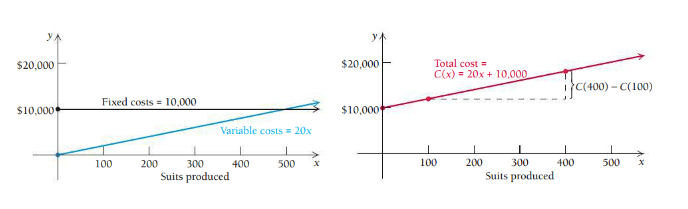
\includegraphics[width=0.85\textwidth]{ marcus.png }
\end{figure}
\bigbreak \noindent
The total-cost function is shown in the graph on the right. From a practical standpoint, the domains of these functions are nonnegative integers.
\bigbreak \noindent
\prob{b} The total cost of producing 100 suits is:
$$ C(100) 20 \cdot 100 + 10,000 = \$12,000$$
\vspace{2mm}

\noindent
The total cost of producing 400 suits is:
$$C(400) = 20 \cdot 400 + 10,000 = \$18,000$$
\bigbreak \noindent \bigbreak \noindent
\subsection{Section Summary}
\begin{minipage}{0.45\textwidth}
  \begin{itemize}
    \item The slope $m$ of a line containing the points $\left(x_1, y_1\right)$ and $\left(x_2, y_2\right)$ is given by $m=\frac{y_2-y_1}{x_2-x_1}$.
    \item  The slope of a line can be interpreted as $\frac{\text { change in } y}{\text { change in } x}$.
    \item A horizontal line has slope $m=0$, and a vertical line has an undefined slope.
  \end{itemize}
\end{minipage}
\begin{minipage}{0.45\textwidth}
  \begin{itemize}
    \item Graphs of functions that are straight lines (linear functions) are characterized by an equation of the type $f(x)=m x+b$, where $m$ is the slope and $(0, b)$ is the $y$-intercept, the point at which the graph crosses the $y$-axis.
    \item The form $y=m x+b$ is called the slope-intercept equation of a line.
    \item The point-slope equation of a line is $y-y_1=m\left(x-x_1\right)$, where $\left(x_1, y_1\right)$ is a point on the line and $m$ is the slope.
\end{itemize}
\end{minipage}
\pagebreak
\section{R.5 Nonlinear Functions and Models}  
\bigbreak \noindent
\thmcon{
  \textbf{\underline{Quadratic Functions}}
  \vspace{3mm}

  A \textbf{quadratic function} is given by
  $$f(x) = ax^2 +bx + c, \hspace{7mm} \text{where } a\neq 0$$
  \bigbreak \noindent
  The graph of a quadratic function is given by $f(x) = ax^2 + bx+c$, where $a\neq 0$ is called a \textbf{parabola}.
  \begin{itemize}
    \item It is always a cup-shaped curve 
    \item It opens upward if $a > 0$ and opens downward if $a < 0$.
    \item Its turning point, or \textbf{vertex} has a first coordinate given by $x= -\frac{b}{2a}$
    \item The vertical line $x = -\frac{b}{2a}$ is the \textbf{line of symmetry}, although it is not part of the graph.
  \end{itemize}
}
\bigbreak \noindent \bigbreak \noindent
\ex{}{
  Graph $f(x) = x^2 - 2x - 3$, and determine and label the vertex and the line of symmetry.
}
\bigbreak \noindent
\sol{}
\vspace{2.5mm}

$$ a=1 \hspace{5mm} b=-2 \hspace{5mm} c= -3$$

The x-coord of the vertex is:

$$ x = -\frac{-2}{2(1)} = 1$$

sub in 1 for x:

$$1^2 - 2(1) -3 = -4$$

So,
$$\text{Vetex: } (1, -4)$$

Solve for x:

$$ (x+1)(x-3) = 0 \hspace{3mm}\rightarrow \hspace{3mm} x=-1, 3 \hspace{3mm}\rightarrow \hspace{3mm} \text{x-ints } (-1,0) , (3,0)$$

Solve for y:

$$ 0^2 - 2(0)-3 \hspace{3mm} \rightarrow \hspace{3mm} \text{y-int } (0,-3)$$

Therfore:

$$ \text{line of symmetry: } x = 1 \hspace{5mm} \text{Vetex: } (-1, 4)\hspace{5mm} \text{x-ints: }(-1,0),(3,0) \hspace{5mm} \text{y-int: }(0,-3)$$
    \begin{center}
  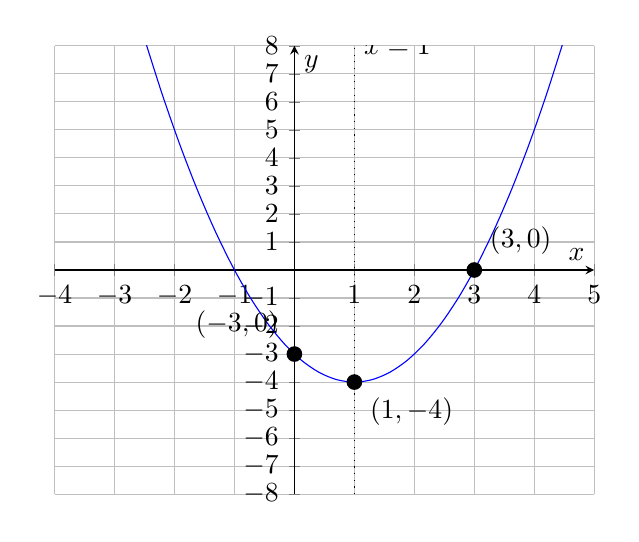
\begin{tikzpicture}
    \begin{axis}[
      axis lines=center,
      xlabel={$x$},
      ylabel={$y$},
      xmin=-4,
      xmax=5,
      ymin=-8,
      ymax=8,
      xtick={-4, -3, -2, -1, 0, 1, 2, 3, 4, 5},
      ytick={-8, -7, -6, -5, -4, -3, -2, -1, 0, 1, 2, 3, 4, 5, 6, 7, 8},
      grid=both,
    ]
      
    % Plot the quadratic function
    \addplot[domain=-2.5:4.5,smooth,blue] {x^2 - 2*x - 3};
    
    % Line of symmetry
    \draw[dotted] (1,-8) -- (1,8) node[right] at (1,8) {$x = 1$};
    
    % Intercepts with labels and filled circles
    \node[fill=black,circle,inner sep=2pt,label={above right:{$(3, 0)$}}] at (3,0) {};
    \node[fill=black,circle,inner sep=2pt,label={above left:{$(-3, 0)$}}] at (0,-3) {};
    
    % Vertex
    \node[fill=black,circle,inner sep=2pt,label={below right:{$(1, -4)$}}] at (1,-4) {};
    
    \end{axis}
  \end{tikzpicture}
    \end{center}
\bigbreak \noindent \bigbreak \noindent
\nt{
  When factoring to solve for the x intercepts seems difficult, we use the \textbf{quadradic formula}
  \vspace{3mm}

  The quadradic formula is given by:

  $$ \frac{-b \pm \sqrt{b^2-4ac}}{2a}$$

}

\bigbreak \noindent
\hrule
\subsection{Algebraic-Graphical Connection}
\bigbreak \noindent
\begin{minipage}{0.5\textwidth}
To make an algebraic-graphical connection  between the solutions of a quadratic equation and the x-intercepts of a quadratic function, consider the graph of $f(x) = x^2+6x+8$ and its x-intercepts shown to the right

The x-intercepts, (-4,0) and (-2,0), are the points of intersection of the graphs of $f(x) = x^2 +6x+8$ and $g(x) = 0$ (the x-axis). The x-values -4 and -2, can be found by solving $f(x) = g(x)$:
$$ x^2+6x+8=0$$
$$(x+4)(x+2) = 0$$
$$x+4 = 0 \text{ \textit{or} } x + 2 = 0$$
$$ x = -4 \text{ \textit{or} } x = -2$$
\end{minipage}
\hfill
\begin{minipage}{0.4\textwidth}
      \centering
  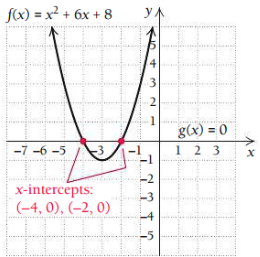
\includegraphics[width=0.8\textwidth]{ graph.png }
\end{minipage}
\bigbreak \noindent \bigbreak \noindent
\hrule
\subsection{Polynomial Functions}
\thmcon{
  \textbf{\underline{Defintion}}
  \vspace{3mm}

  a \textbf{polynomial Function} $f$ is given by
  $$
f(x)=a_n x^n+a_{n-1} x^{n-1}+\cdots+a_2 x^2+a_1 x^1+a_0,
$$

Where $n$ is a nonnegative integer and $a_n$, $a_{n-1}$, \ldots, $a_1$,$a_0$ are real numbers called \textbf{coefficients}.

}
\pagebreak
\centerline{The following are examples of polynomial functions:}
\vspace{3mm}

$$f(x)=-5 \hspace{30mm} (\text{A constant function})$$
$$f(x)=4x+3 \hspace{30mm} (\text{A linear function})$$
$$f(x) = 2x^3 -4x^2+x+1 \hspace{10mm} (\text{A quadratic function})$$
$$f(x) = 2x^3 - 4x^2+x+1 \hspace{10mm} (\text{A cubic function})$$
\bigbreak \noindent \bigbreak \noindent
\ex{}{
  Using the same set of axes, graph $f(x) =x^2$ and $g(x)= x^3$
}
  \begin{center}
    \begin{tikzpicture}
      \begin{axis}[
      restrict y to domain=-10:10,
      restrict x to domain=-10:10,
      samples=200, % 0 if you dont need lines
      xmin=-10,
      xmax=10,
      ymin=-10,
      ymax=10,
      axis lines=middle,
      xlabel={$x$},
      ylabel={$y$},
      %grid=both % Grid lines
      ]
      \addplot[color=red]{x^2};
      \addplot[color=blue]{x^3};
      \end{axis} 
    \end{tikzpicture}
  \end{center}
\bigbreak \noindent \bigbreak \noindent
\hrule
\subsection{Rational Functions}
\bigbreak \noindent
\thmcon{
  \textbf{\underline{Defintion}}
  \vspace{3mm}

  Functions that can be expressed as the quotient, or ratio, of two polynomials are called \textbf{rational functions}
  \bigbreak \noindent
  The following are examples of rational functions
  $$ f(x) = \frac{x^2-9}{x-3} \hspace{10mm} h(x) = \frac{x-3}{x^2-x-2}$$
  $$\hspace{20mm} g(x) = \frac{3x^2 -4x}{2x+10} \hspace{10mm} k(x) = \frac{x^3-2x+7}{1} = x^3-2x+7$$
  \bigbreak \noindent
  As the function $k$ illustrates, every polynomial function is also a rational function.
}
\bigbreak \bigbreak \noindent
\nt{
  y is \textbf{inversely proportional} to x if there is some positive number $k$ for which $y = \frac{k}{x}$
}
\pagebreak
\ex{}{
  A minor league baseball team notices that as the average ticket price increases, the number of tickets sold decreases, and as the average ticket price decreases, the number of tickets sold increases. Suppose 10,000 tickets are sold when the average ticket price is \$12. Assuming that the relationship between average ticket price x, in dollars, and the number of tickets sold y is an inverse proportion, find the number of tickets sold when the average price is \$20.
}
\sol{Assuming that $y=\frac{k}{x}$, we substitue $10,000$ for y and 12 for x to find k}
\vspace{2.5mm}

$$ 10,000 = \frac{k}{12}$$

$$k = 120,000$$
\vspace{2.5mm}

\noindent\textbf{Thus,}
\bigbreak
The inversely proportional relationship is given by y = $\frac{120,000}{x}$
\bigbreak \bigbreak
\noindent \textbf{substituting 20 for x, we have}

$$y=\frac{120,000}{x} = 6000$$
\bigbreak \bigbreak
\noindent \textbf{Therefore:}
\bigbreak
When the average ticket price is \$20, about 6000 tickets will be sold.
\bigbreak \bigbreak
\hrule
\subsection{Absolute-Value Functions}
\bigbreak \noindent
The \textbf{absolute value}  of a number is its distance from 0 on the number line. We denote the absolute value of a number x as $\lvert x \rvert$
\bigbreak \bigbreak \noindent
Graphing $f(x) = \lvert x \rvert$, we get,
\bigbreak
\begin{center}
  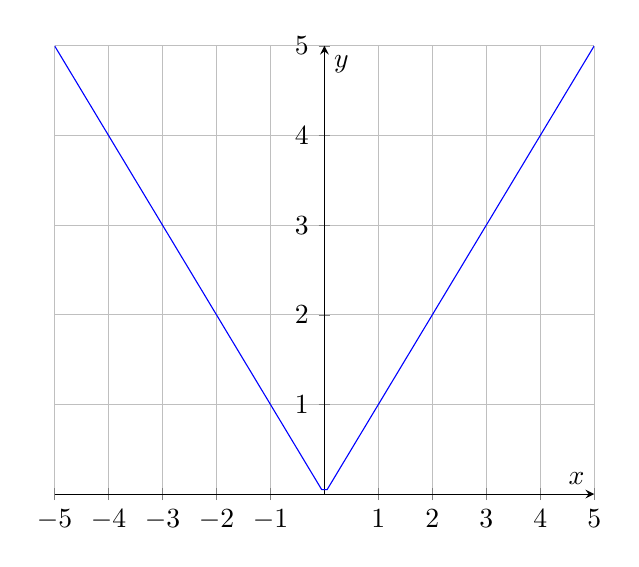
\begin{tikzpicture}
    \begin{axis}[
      axis lines=center,
      xlabel={$x$},
      ylabel={$y$},
      xmin=-5,
      xmax=5,
      ymin=0,
      ymax=5,
      xtick={-5, -4, -3, -2, -1, 0, 1, 2, 3, 4, 5},
      ytick={0, 1, 2, 3, 4, 5},
      grid=both,
    ]
      
    % Plot the absolute value function
    \addplot[domain=-5:5,blue,mark=none,samples=100] {abs(x)};
    
    \end{axis}
  \end{tikzpicture}
\end{center}

\pagebreak
\subsection{Square-Root Functions}
\bigbreak \noindent
The following is an example of a square-root function and its graph.
\bigbreak \noindent \bigbreak \noindent
\begin{figure}[htbp]
\begin{minipage}{0.4\textwidth}
  \hspace{20mm}$f(x) = \sqrt{x}$
\end{minipage}
\begin{minipage}{0.5\textwidth}
  \begin{tikzpicture}
    \begin{axis}[
      axis lines=center,
      xlabel={$x$},
      ylabel={$y$},
      xmin=0,
      xmax=3,
      ymin=0,
      ymax=3,
      xtick={0, 1, 2, 3},
      ytick={0, 1, 2, 3},
      grid=both,
    ]
      
    % Plot the square root function
    \addplot[domain=0:3,blue,mark=none,samples=100] {sqrt(x)};
    
    \end{axis}
  \end{tikzpicture}
\end{minipage}
\end{figure}
\bigbreak \noindent \bigbreak \noindent 
\section*{R.6 - Exponential and logarithmic Funcitons}
\bigbreak \noindent
\begin{minipage}{0.5\textwidth}
Every term in a polynomial function can be written in the form of a variable raised to a power. Here we consider exponential functions, in which the exponent is a variable (or an expression containing a variable). Exponential functions are used to model real-word problems that include heating/cooling rates, population growth and decay, compound interest, and much more. Every exponential function has the property that it outputs change at a rate that is a constant percentage
\end{minipage}
\hspace{10mm}\begin{minipage}{0.4\textwidth}
\thmcon{
  \textbf{\underline{Defintion}}
  \vspace{3mm}

  An exponential function $f$ is given by
  $$f(x) = a_0 \cdot x^x$$
  \vspace{2mm}

  where x is any real number and $a > 0$ and $a \neq 1$. The number $a$ is the base and the y-intercept is $(0,a_0)$
}	
\end{minipage}
\bigbreak \noindent \bigbreak \noindent
The following are examples of exponential functions:

$$ f(x) = 2^x, \hspace{10mm} f(x) = \left(\frac{1}{2}\right)^x, \hspace{10mm} f(x) = 3(0.4)^x$$
\bigbreak \noindent
\nt{
  Note that in contrast to a power function like $y = x^2$, an exponential function has the variable in the exponent, not the base.
}
\pagebreak
\ex{}{
  Graph $y = f(x) = \left(\frac{5}{4}\right)^x = 1.25^x$
}
\bigbreak \noindent
\begin{figure}[htbp]
\begin{minipage}{0.5\textwidth}
First, we find some function values. \\ Note that $1.25^x$ is always positive.  

\vspace{2mm}

$x=-3, \hspace{3mm} y=1.25^{-3} = \frac{64}{125}$
\vspace{2mm}

$x=-2 \hspace{3mm} y=1.25^{-2} = \frac{16}{25}$
\vspace{2mm}

$x=-1 \hspace{3mm}y=1.25^{-1}= \frac{4}{5}$
\vspace{2mm}

$x=0 \hspace{3mm} y= 1.25^0 = 1$
\vspace{2mm}

$x=1 \hspace{3mm} y= 1.25^1 = \frac{5}{4}$
\vspace{2mm}

$x=2 \hspace{3mm} y=1.25^2 = \frac{25}{16}$
\vspace{2mm}

$x=3 \hspace{3mm}y=1.25^3 \frac{125}{64}$
\end{minipage}
\begin{minipage}{0.45\textwidth}
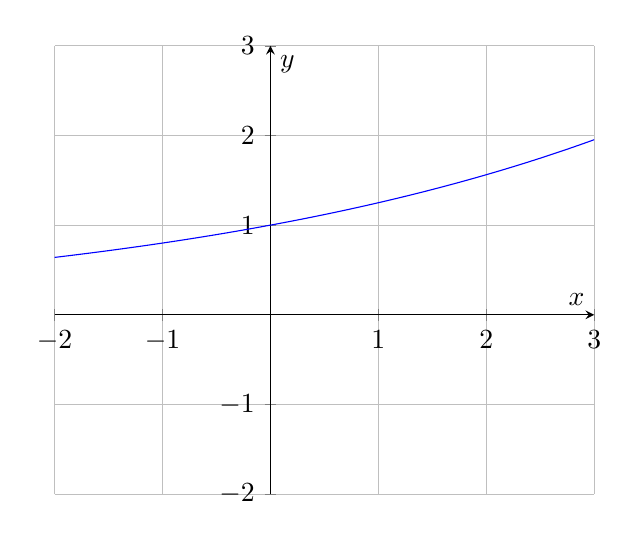
\begin{tikzpicture}
    \begin{axis}[
      axis lines=center,
      xlabel={$x$},
      ylabel={$y$},
      xmin=-2,
      xmax=3,
      ymin=-2,
      ymax=3,
      xtick={-2,-1,0, 1, 2, 3},
      ytick={-2,-1,0, 1, 2, 3},
      grid=both,
    ]
    \addplot[domain=-2:3,blue,mark=none,samples=100] {1.25^x};
    \end{axis}
  \end{tikzpicture}
\end{minipage}
\end{figure}
\bigbreak \noindent \bigbreak \noindent
\ex{}{
  Graph: $f(x) = 3\cdot \left(\frac{1}{4}\right)^x$
}
\bigbreak\noindent\bigbreak\noindent
\begin{figure}[ht]
    \centering
    %\caption{figure2}
    %\label{fig:figure2}
  \end{figure}
  \begin{minipage}{0.4\textwidth}
  We find some values:	
  \vspace{2mm}

  $x=-3\hspace{3mm} y=3\cdot \left(\frac{1}{4}\right)^-3 = 192$
  \vspace{2mm}

  $x=-2 \hspace{2mm}y=3\cdot \left(\frac{1}{4}\right)^-2 = 48$
  \vspace{2mm}

  $x=-1\hspace{2mm}y=3\cdot \left(\frac{1}{4}\right)^-1 = 12$
  \vspace{2mm}

  $x=0\hspace{2mm}y=3\cdot \left(\frac{1}{4}\right)^0 = 3$
  \vspace{2mm}

  $x=1\hspace{2mm}y=3\cdot \left(\frac{1}{4}\right)^1 = \frac{3}{4}$
  \vspace{2mm}

  $x=2\hspace{2mm}y=3\cdot \left(\frac{1}{4}\right)^2=\frac{3}{16}$
  \vspace{2mm}

  $x=3\hspace{2mm}y=3\cdot \left(\frac{1}{4}\right)^ = \frac{3}{64}$
  \end{minipage}
\begin{minipage}{0.5\textwidth}
    \incfig[1]{figure2}
\end{minipage}
\pagebreak
\ex{}{
  Bert invests $10,000$ in an account that earns 3.25\% interest per year
  \vspace{3mm}

  \textbf{a)} Find the function that gives the value A of Bert's investment after t years
  \vspace{3mm}

  \textbf{b)} Find A(10), and interpret this result.
  \vspace{3mm}

  \textbf{c)} Graph A(t) for 0 $\le t \le 10$
}
\bigbreak\noindent
\sol
\bigbreak
\noindent We know that the amount $P$ invested at interest rate $r$, compounded annually for t years, grows to an amount A, given by
$$ A = P(1+r)^t$$

\noindent For $P = \$10,000$ and $r = 3.25\% = 0.0325$, we have
$$A = 10,000(1.0325)^t$$
\bigbreak \noindent
For A(10) we have,
$$ A(10) = 10,000(1.0325)^10$$
$$ = 13,768.94$$
\bigbreak \noindent
The graph is shown below
\bigbreak 
\begin{figure}[ht]
    \centering
    \incfig[1]{bert}
    %\caption{bert}
    %\label{fig:bert}
\end{figure}
\pagebreak
\ex{}{
  The city of Cuprite had a population of 15,000 people in 2012, when the closing of a mine initiated a decrease in population that persisits to the present. Assume that the population decreases by the same percentage every year and that in 2017 the population was 11,250
  \bigbreak \noindent
  a) Find $P(t)$, the population of Cuprite $t$ years after 2012 .
  \bigbreak \noindent
b) Estimate Cuprite's population in 2022.
\bigbreak \noindent
c) Graph $P(t)$ for $0 \leq t \leq 10$.
\bigbreak \noindent
d) Find the annual percent change in Cuprite's population.
}
\bigbreak \noindent
\sol
\bigbreak \noindent
since we know that after 5 years, the population was at 11,250, we can use t = 5
$$11,250 = 15,000(a)^5$$
$$11,250 = 15,000a^5 \rightarrow \frac{11,250}{15,000} = a^5$$
$$\left(\frac{11,250}{15,000}\right)^{\frac{1}{5}} = a$$

$$a \approx 0.944$$
\bigbreak \noindent
Thus our function for the model is $$P(t) = 15,000(0.944)^t$$
\bigbreak \noindent 
Therefore in 2022, the estimated population will be
$$P(10) = 15,000(0.944)^{10} \approx 8430$$
\bigbreak \noindent
The graph is shown below
\bigbreak \noindent
\begin{figure}[ht]
    \centering
    \incfig[1]{pop}
    %\caption{pop}
    %\label{fig:pop}
\end{figure}
\pagebreak
\subsection*{\LARGE{Logarithms}}
\bigbreak \noindent
\begin{mdframed}
\begin{minipage}{0.5\textwidth}
  a \textbf{logarithm} is an exponent. For example, because $3^2 + 9 $, we say ``the logarithm base 3, of 9 is 2.'' Using logarithm notation we write
  $$\log_39=2$$
  \vspace{3mm}
  
  In general, if $a^x = y$, then $\log_ay=x$
\end{minipage}
\hspace{10mm}\begin{minipage}{0.4\textwidth}
  \vspace{3mm}

\thmcon{
  \textbf{\underline{Defintion}}
  \vspace{8mm}

  The \textbf{logarithm} base $a$ of $y$ is the number $x$ for which $a^x = y$
  \vspace{3mm}

  Equivalently, $a^x = y$, if and only if $\log_ay =x$
  \vspace{3mm}

  The base $a$ must be positive and not equal to 1, that is $a>0$ and $a \neq 1$
}	
\vspace{2mm}
\end{minipage}
\end{mdframed}
\bigbreak \noindent  
We can rewrite exponential equations as equivalent logarithmic equations, and logarithmic equations as equivalent exponential equations.
\bigbreak \noindent
\ex{}{
  Rewrite each exponential equation as an equivalent logarithmic equation:

  $$a) \ 2^5 = 32 \hspace{6mm} b) \ 4^2 = 16 \hspace{6mm} c)\ 6^1 = 6 \hspace{6mm} d)\ 3^{-2} = \frac{1}{9} \hspace{6mm} e) \ 7^0 = 1$$
}
\bigbreak \noindent
\sol
\bigbreak \noindent
We use the definition of logarithms: The logarithm, base a, of y is the number x for which $a^x = y$
\bigbreak \noindent
a) Since $2^5 = 32$, we have $\rightarrow \log_232=5$
\bigbreak \noindent
b) Since $4^2 = 16$. we have $ \rightarrow \log_416=2$
\bigbreak \noindent
c) Since $6^1 = 6$, we have $\log_6 = 1$
\bigbreak \noindent
d) Since, $3^{-2} = \frac{1}{9}$, we have $\rightarrow \log_3\left(\frac{1}{9}\right) = -2$
\bigbreak \noindent
e) Since $7^0 = 1$, we have $\log_71=0$
\bigbreak \noindent
\ex{}{
  Rewrite each logarithmic equation as an equivalent exponential equation:
$$ a) \ \log_525 = 2 \hspace{8mm} b) \ \log_3243=5\hspace{8mm} c)\ \log_{10}100=2\hspace{8mm} d) \ \log_40.25=-1$$
}
\bigbreak \noindent
\sol
We use the definition of logarithms, base a, of y is the number x for which $a^x=y$
\bigbreak \noindent
a) since $\log_525 = 2$, we identify the base as 5 and the exponent as 2. Thus, we have $5^2 = 25$.
\bigbreak \noindent
b) Since $\log_3243 = 5$, we have $3^5 = 243$
\bigbreak \noindent
c) Since $\log_{10}100=2$, we have $10^2 = 100$
\bigbreak \noindent
d) Since $\log_4.025 = -1$, we have $4^{-1} = 0.25$
\pagebreak
\subsection*{Basic Properties of Logarithms}
\bigbreak \noindent
\begin{mdframed}
\begin{minipage}{0.4\textwidth}
The following are some basic properties of logarithms. Properties P4, P5, P7, and P8 follow directly from the definition of a logarithm.	
\end{minipage}
\hspace{8mm}\begin{minipage}{0.5\textwidth}
  \thm{}{
  P1. $\log _a(M N)=\log _a M+\log _a N$
  \vspace{3mm}

P2. $\log _a\left(\frac{M}{N}\right)=\log _a M-\log _a N$
  \vspace{3mm}

P3. $\log _a\left(M^b\right)=b \log _a M$
  \vspace{3mm}

P4. $\log _a a=1$
  \vspace{3mm}

P5. $\log _a 1=0$
  \vspace{3mm}

P6. $\log _a M=\frac{\log _b M}{\log _b a}$ (the change-of-base formula)
  \vspace{2mm}

P7. $\log _a a^h=k$
  \vspace{3mm}

P8. For any $x>0, a^{\log _a x}=x$.
	}
\end{minipage}
\end{mdframed}
\bigbreak \noindent
\ex{}{
  Given
  $$ log_a 2 = 0.301 \hspace{6mm} \text{and} \hspace{6mm} log_a3 = 0.477$$
  Find each of the following 
  \bigbreak \noindent
  a) $\log _a 6$; \hspace{4mm}
b) $\log _a \frac{2}{3}$;\hspace{4mm}
c) $\log _a 81$; \hspace{4mm}
d) $\log _a \frac{1}{3}$;
\vspace{3mm}

e) $\log _a \sqrt{a}$\hspace{4mm}
f) $\log _a(2 a)$;\hspace{4mm}
g) $\frac{\log _a 3}{\log _a 2}$\hspace{4mm}
h) $\log _a 5$.
}
\bigbreak \noindent
\begin{minipage}{0.5\textwidth}
\text { a) } 
$$\log _a 6  =\log _a(2 \cdot 3)$$
 $$=\log _a 2+\log _a 3 $$
$$ =0.301+0.477 $$
 $$=0.778$$
 \bigbreak \noindent
b)
$$\log _a \frac{2}{3}  =\log _a 2-\log _a 3$$
 $$=0.301-0.477 $$
$$ =-0.176$$

c)
$$\log _a 81  =\log _a 3^4 $$
 $$=4 \log _a 3 $$
$$ =4(0.477) $$
$$ =1.908$$
\end{minipage}
\begin{minipage}{0.4\textwidth}
d)
$$\log _a \frac{1}{3}  =\log _a 1-\log _a 3 $$
$$ =0-0.477 $$
$$ =-0.477$$
\bigbreak \noindent
e) $\log _a \sqrt{a}=\log _a\left(a^{1 / 2}\right)=\frac{1}{2}$
\bigbreak \noindent
f)
$$\log _a(2 a)  =\log _a 2+\log _a a $$
$$ =0.301+1 $$
$$ =1.301$$
\bigbreak \noindent
g) $\frac{\log _a 3}{\log _a 2}=\frac{0.477}{0.301} \approx 1.58$
\end{minipage}
\pagebreak
\subsection*{Common Logarithms}
The number $\log_{10}x$ is the common logarithm of x and is abbreviated as $\log x$
\bigbreak \noindent
\thmcon{
  \textbf{\underline{Defintion}}
  \vspace{3mm}

  For any positive number $x$, $\log x = \log_{10} x$
}
\bigbreak \noindent 
Thus, when we write ``$\log x$'' with no base indicated, base 10 is assumed. Note the following comparisons of common logarithms and powers of 10.
\bigbreak \noindent
\ex{}{
  Use common logarithms and the change of base formula to find the following:
  $$a) \log 45 \hspace{10mm} \log_5 12 \hspace{10mm} \log_6 27$$
}
\sol 
\bigbreak \noindent
a) $\log 45 = \frac{\log 45}{\log 10} \approx 45$
\bigbreak \noindent
b) $\log_5 12 = \frac{\log 12}{\log 5} \approx 12$
\bigbreak \noindent
c) $\log_6 27 = \frac{\log 27}{\log 6} \approx 27$
\bigbreak \noindent \bigbreak \noindent
\subsection*{Graphs of Logarithmic Functions}
\bigbreak \noindent
The graph of a logarithmic function of the form $g(x) = \log_a x $ can be drawn by considering the graph of $f(x) = a^x$ and reversing the coordinates in each ordered pair. For example, the graph of $f(x) = 2^x$ is shown below, along with an input-output table.
\bigbreak \noindent \bigbreak \noindent
\begin{minipage}{0.5\textwidth}
	\begin{tabular}{|c|c|c|c|c|c|c|c|}
\hline$x$ & -3 & -2 & -1 & 0 & 1 & 2 & 3 \\
\hline$y=f(x)=2^x$ & $\frac{1}{8}$ & $\frac{1}{4}$ & $\frac{1}{2}$ & 1 & 2 & 4 & 8 \\
\hline
\end{tabular}
\end{minipage}
\begin{minipage}{0.45\textwidth}
    \incfig[1]{log}
\end{minipage}
\pagebreak
\noindent
\begin{large}
  To graph $g(x) = \log_2 x$ we reverse the coordinates of each ordered pair:
\end{large}
\bigbreak \noindent \bigbreak \noindent
\begin{minipage}{0.5\textwidth}
 \begin{tabular}{|c|c|c|c|c|c|c|c|}
\hline$x$ & $\frac{1}{8}$ & $\frac{1}{4}$ & $\frac{1}{2}$ & 1 & 2 & 4 & 8 \\
\hline$y=g(x)=\log _2 x$ & -3 & -2 & -1 & 0 & 1 & 2 & 3 \\
\hline
\end{tabular} 
\end{minipage}
\begin{minipage}{0.45\textwidth}
    \incfig[1]{log2}
\end{minipage}
\bigbreak \noindent \bigbreak \noindent
\nt{
  All functions of the form $g(x) = \log_a x$, where $ a>1$, have the following characteristics.
  \bigbreak \noindent
  \begin{itemize}
    \item The domain is $\{x \mid x>0\}$.
\item The range is $\{y \mid-\infty<y<\infty\}$.
\item The $x$-intercept is $(1,0)$.
\item There is no $y$-intercept.
\item As $x$ approaches infinity, so does $y$, but more slowly.
\item  As $x$ approaches $0, y$ decreases toward negative infinity.
\end{itemize}
}
\bigbreak \noindent \bigbreak \noindent
\ex{}{
  Bert deposits \$20,000 in a savings account that earns 3.25\% interest per year. When will his account have a value of \$20,000?
}
\sol
\bigbreak \noindent
$$A(t) = 10,000(1.0325)^t$$

$$ 20,000 = 10,000(1.0325)^t $$
$$ 2 = (1.0325)^t$$
$$t = \log_{1.0325}2$$
$$t = \frac{\log 2}{\log_{1.0325}} \approx 21.67$$
\bigbreak \noindent \bigbreak \noindent
Berts savings account will reach a value of \$20,000 after about 21.67 yr.
\end{document}
